\documentclass{article}

\usepackage{fancyhdr}
\usepackage{extramarks}
\usepackage{amsmath}
\usepackage{amssymb}
\usepackage{amsthm}
\usepackage{amsfonts}
\usepackage{tikz}
\usepackage[noend]{algpseudocode}
\usepackage{algorithmicx,algorithm}
\usepackage{algpseudocode}
\usepackage{enumerate}
\usepackage{color}
\usetikzlibrary{automata,positioning}

%
% Basic Document Settings
%

\topmargin=-0.45in
\evensidemargin=0in
\oddsidemargin=0in
\textwidth=6.5in
\textheight=9.0in
\headsep=0.25in

\linespread{1.1}

\pagestyle{fancy}
\lhead{\hmwkAuthorName}
\chead{\hmwkClass}
\rhead{\hmwkTitle}
\lfoot{\Address}
\rfoot{Page \thepage}
\cfoot{}

\renewcommand\headrulewidth{0.4pt}
\renewcommand\footrulewidth{0.4pt}

\setlength\parindent{0pt}

%
% Create Problem Sections
%

\newcommand{\enterProblemHeader}[1]{
    \nobreak\extramarks{}{Problem \arabic{#1} continued on next page\ldots}\nobreak{}
    \nobreak\extramarks{Problem \arabic{#1} (continued)}{Problem \arabic{#1} continued on next page\ldots}\nobreak{}
}

\newcommand{\exitProblemHeader}[1]{
    \nobreak\extramarks{Problem \arabic{#1} (continued)}{Problem \arabic{#1} continued on next page\ldots}\nobreak{}
    \stepcounter{#1}
    \nobreak\extramarks{Problem \arabic{#1}}{}\nobreak{}
}

\setcounter{secnumdepth}{0}
\newcounter{partCounter}
\newcounter{homeworkProblemCounter}
\setcounter{homeworkProblemCounter}{1}
\nobreak\extramarks{Problem \arabic{homeworkProblemCounter}}{}\nobreak{}

\newenvironment{homeworkProblem}{
    \section{Problem \arabic{homeworkProblemCounter}}
    \setcounter{partCounter}{1}
    \enterProblemHeader{homeworkProblemCounter}
}{
    \exitProblemHeader{homeworkProblemCounter}
}

%
% Homework Details
%   - Title
%   - Due date
%   - Class
%   - Section/Time
%   - Instructor
%   - Author
%

\newcommand{\hmwkTitle}{Assignment\#4}
\newcommand{\hmwkDueDate}{\today}
\newcommand{\hmwkClass}{Pattern Recognition}
\newcommand{\hmwkClassTime}{}
\newcommand{\Address}{SSE TongJi University}
\newcommand{\hmwkClassInstructor}{Professor Ying Shen}
\newcommand{\hmwkAuthorName}{2031566/Yang Han}

%
% Title Page
%

\title{
    \vspace{2in}
    \textmd{\textbf{\hmwkClass\\ \hmwkTitle}}\\
    \normalsize\vspace{0.1in}\small{By\ \textit{\hmwkClassInstructor\ \hmwkClassTime }}\\
 %   \vspace{0.1in}\small{\Address \\ Due\ on\ \hmwkDueDate\  }
    \vspace{3in}
}

\author{\textbf{\hmwkAuthorName}}
\date{\today}

\renewcommand{\part}[1]{\textbf{\large Part \Alph{partCounter}}\stepcounter{partCounter}\\}

%
% Various Helper Commands
%

% Useful for algorithms
\newcommand{\alg}[1]{\textsc{\bfseries \footnotesize #1}}

% For derivatives
\newcommand{\deriv}[1]{\frac{\mathrm{d}}{\mathrm{d}x} (#1)}

% For partial derivatives
\newcommand{\pderiv}[2]{\frac{\partial}{\partial #1} (#2)}

% Integral dx
\newcommand{\dx}{\mathrm{d}x}

% Alias for the Solution section header
\newcommand{\solution}{\textbf{\large Solution}}

% Probability commands: Expectation, Variance, Covariance, Bias
\newcommand{\E}{\mathrm{E}}
\newcommand{\Var}{\mathrm{Var}}
\newcommand{\Cov}{\mathrm{Cov}}
\newcommand{\Bias}{\mathrm{Bias}}

\begin{document}
	\maketitle
	\newpage

	\section*{1 Introduction} % Unnumbered section
	In this assignment, I will implement KMeans and use it to cluster Seeds Data Set \((http://archive.ics.uci.edu/ \\
	ml/datasets/seeds)\) and Iris Data Set\((http://archive.ics.uci.edu/ml/datasets/Iris)\).

		\subsection{1.1 Seeds Dataset}
			The dataset belongs to three different varieties of wheat and is consisted of seven geometric parameters, 1. area A,
			2. perimeter P,
			3. compactness C
			4. length of kernel,
			5. width of kernel,
			6. asymmetry coefficient
			7. length of kernel groove. All of these parameters were real-valued continuous.

		\subsection{1.2 Iris Dataset}
			Iris Dataset is perhaps the best known database to be found in the pattern recognition literature, 
			The data set contains 3 classes of 50 instances each, where each class refers to a type of iris plant.
			One class is linearly separable from the other 2; the latter are NOT linearly separable from each other.

	\section{2 Data Preprocess}
	As I show in the $preprocess.ipynb$ file, I mainly do three things:
		\begin{enumerate}[1.]
			\item Read the raw file content, cast the str type to float type save save them to csv format.
			\item Map categories to ordered numbers(eg. 0,1,2...).
			\item In order to eliminate the dimensional influence between indicators, data standardization
				is required to solve the comparability between data indicators.
		\end{enumerate}

	\section{3. Program Modules}

		\subsection{3.1 Theory}
			The main element of k-means algorithm works by a two-step process called expectation-maximization.
			The expectation step assigns each data point to its nearest centroid.
			Then, the maximization step computes the mean of all the points for each cluster and sets the new centroid.
			The main algorithm was described as below:

			\begin{algorithm}
				\caption{K-means algorithm}
				\hspace*{0.02in}
				\begin{algorithmic}[1]
					\State Specify the number k of clusters to assign.
					\State Randomly initialize k centroids.
					\Repeat
						\State \textbf{expectation: } Assign each point to its closest centroid.
						\State \textbf{maximization: } Compute the new centroid(mean) of each cluster.
					\Until The centroid positions do not change or iteration reach the max iteration times(30).
				\end{algorithmic}
			\end{algorithm}
		
		\subsection{3.2 Code}
			In the assignment, I follow the scikit-learn style to design my KMeans class which accepts one parameter name $n\_clusters$ with
			default value as 2. The two main methods name $fit$ and $predict$, $fit$ accepts the samples and execute the k-means algorithm, 
			$predict$ doesn't accept parameter and return the labels of each sample.

	\section{4. Result}
		In Seeds Data Set, I set $n\_clusters=3$, and get a result as below:
			\begin{figure}[H]
				\centering
				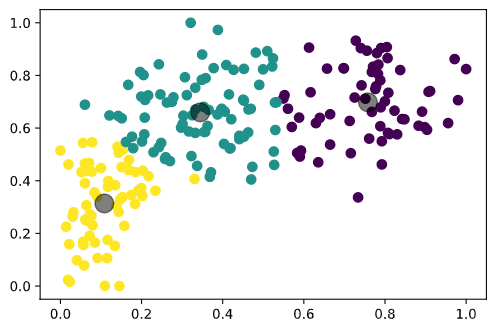
\includegraphics[width=0.6\textwidth]{1.png}
				\caption{Seeds Data Set cluster}
				\label{Fig.main5}
			\end{figure}

		In Iris Data Set, I set $n\_clusters=3$, and get a result as below:
			\begin{figure}[H]
				\centering
				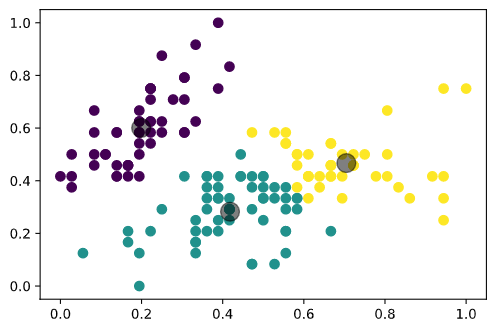
\includegraphics[width=0.6\textwidth]{2.png}
				\caption{Iris Data Set cluster}
				\label{Fig.main5}
			\end{figure}

	\section{Limitations and Inprovements}
		The KMeans algorithm is nondeterministic, meaning it could produce different results from two separate runs
		even if the runs were based on the same input. Instead we can use $DBSCAN$ to get a stable result.

\end{document}